% Interface Assumption schematic illustration.
%
% Provenance: this figure is bound by ci/illustration_lineage.json
% to the Interface Assumption block in main.tex (lines 253-257).
% The block is text-only in the body; this schematic is a reviewer
% aid that exposes the dataflow:
%
%   text in -> (frozen encoder Phi) -> per-token displacement <= L
%            -> text out -> deterministic verifier -> pass/fail
%
% Claim scope: schematic illustration only; not empirical evidence.
% The certificate (L14) verifies that the source LaTeX block has
% not drifted relative to when this figure was authored.

\begin{figure}[!htb]
\centering
\resizebox{\linewidth}{!}{%
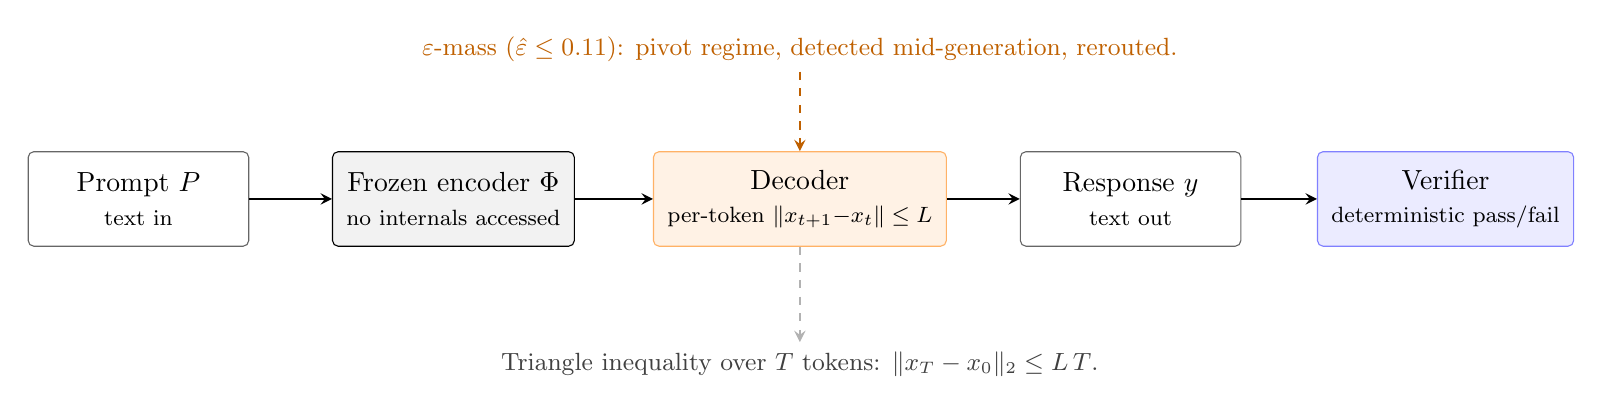
\begin{tikzpicture}[
    font=\normalsize,
    box/.style={draw, rounded corners=2pt, minimum height=12mm, minimum width=28mm, align=center, inner sep=5pt},
    encbox/.style={box, fill=gray!10},
    verbox/.style={box, fill=blue!8, draw=blue!50},
    iobox/.style={box, fill=white, draw=black!60},
    arr/.style={->, thick, >=stealth},
    annot/.style={font=\small, color=black!75},
]
    % Top row: data flow
    \node[iobox] (prompt) at (0, 0) {Prompt $P$\\\footnotesize text in};
    \node[encbox] (enc) at (4.0, 0) {Frozen encoder $\Phi$\\\footnotesize no internals accessed};
    \node[box, fill=orange!10, draw=orange!60] (gen) at (8.4, 0) {Decoder\\\footnotesize per-token $\|x_{t+1}{-}x_t\| \le L$};
    \node[iobox] (out) at (12.6, 0) {Response $y$\\\footnotesize text out};
    \node[verbox] (ver) at (16.6, 0) {Verifier\\\footnotesize deterministic pass/fail};

    \draw[arr] (prompt) -- (enc);
    \draw[arr] (enc) -- (gen);
    \draw[arr] (gen) -- (out);
    \draw[arr] (out) -- (ver);

    % Bottom annotation: the bound that follows
    \node[annot] (bound) at (8.4, -2.1) {%
        Triangle inequality over $T$ tokens: $\|x_T - x_0\|_2 \le L\,T$.
    };
    \draw[arr, dashed, gray!60] (gen) -- (bound);

    % Pivot regime callout (more readable: small + dark orange, not italic gray)
    \node[annot, color=orange!75!black] (pivot) at (8.4, 1.9) {%
        $\varepsilon$-mass ($\hat\varepsilon \le 0.11$): pivot regime, detected mid-generation, rerouted.%
    };
    \draw[arr, dashed, orange!75!black] (pivot) -- (gen);
\end{tikzpicture}
}
\caption{Interface Assumption (schematic): text-in / text-out, frozen encoder, deterministic verifier. The Lipschitz bound $\|x_{t+1}{-}x_t\|\le L$ on per-token displacement is the contract; integrating over $T$ tokens gives $\|x_T - x_0\|\le LT$. The $\varepsilon$-mass (11\%) is the pivot regime detected mid-generation and rerouted (Appendix~\ref{app:direction_stability}). Provenance for this illustration: \texttt{ci/illustration\_lineage.json}; the certificate fails if the source assumption text drifts.}
\label{fig:interface_assumption}
\end{figure}
